%--------------------
% Packages
% -------------------
\documentclass[10pt,letter]{article}
\usepackage[utf8x]{inputenc}
\usepackage[T1]{fontenc}
%\usepackage{gentium}
\usepackage{mathptmx} % Use Times Font
% \usepackage[siunitx]{circuitikz} % for circuit schematics
\usepackage{siunitx}
\usepackage{amsmath} % for the equation* environment


\usepackage[pdftex]{graphicx} % Required for including pictures % clashes with circuitikz
% \usepackage[swedish]{babel} % Swedish translations
\usepackage[pdftex,linkcolor=black,pdfborder={0 0 0}]{hyperref} % Format links for pdf
\usepackage{calc} % To reset the counter in the document after title page
\usepackage{enumitem} % Includes lists

\frenchspacing % No double spacing between sentences
\linespread{1.2} % Set linespace
\usepackage[a4paper, lmargin=0.1666\paperwidth, rmargin=0.1666\paperwidth, tmargin=0.1111\paperheight, bmargin=0.1111\paperheight]{geometry} %margins
%\usepackage{parskip}

\usepackage[all]{nowidow} % Tries to remove widows
\usepackage[protrusion=true,expansion=true]{microtype} % Improves typography, load after fontpackage is selected

\usepackage[inkscapelatex=false]{svg}
\graphicspath{ {./media/} }


%-----------------------
% Set pdf information and add title, fill in the fields
%-----------------------
\hypersetup{ 	
pdfsubject = {},
pdftitle = {ee5311-2025-ee24s053-pwc-report-tut2},
pdfauthor = {Karthik B K <ee24s053@smail.iitm.ac.in>}
}

%-----------------------
% Begin document
%-----------------------
\begin{document}

\title{EE5311 \\ Report of Practical Work Conducted for Tutorial 02}
\author{Karthik B K ee24s053}
\maketitle

\section{Experiment 01}
\subsection{Calculations}
In the given circuit schematic, we know from visual inspection that the pMOS's region of operation will be \emph{saturation} and that of the nMOS will be \emph{linear}. With that information, we equate the currents in the said regions of operations as follows:

\begin{center}
    $I_{d,sat,p} = I_{d,lin,n}$ \\
    $\frac{1}{2}\mu_{p}C_{ox}(\frac{W}{L})_{p}\frac{E_{C}(V_{gs}-V_{tp})^{2}}{V_{gs}-V_{tp}+E_{C}}(1+\lambda_{p} V_{ds}) = \frac{1}{2}\mu_{n}C_{ox}(\frac{W}{L})_{n}\frac{1}{1+(\frac{V_{ds}}{E_{C}})}(2(V_{gs}-V_{tn})V_{ds}-V_{ds}^2)(1+\lambda_{n} V_{ds})$
\end{center}

We use the values provided in the problem statement, and obtain:

\begin{center}
    $(\frac{W}{L})_{p} = 1.610$
\end{center}

Since the minimum width of a 3-terminal pMOS transistor in the given sky130 standard cell library is $0.42 \mu m$, we want to increase the length of our pMOS device to meet this aspect ratio. Hence, we would size the pMOS transistor as follows:

\begin{center}
    $W_{p} = 0.42 \mu m, L_{p} = 0.26 \mu m$
\end{center}

\subsection{Schematics}
We draw the following schematic using \emph{xschem}.
\newline
\begin{center}
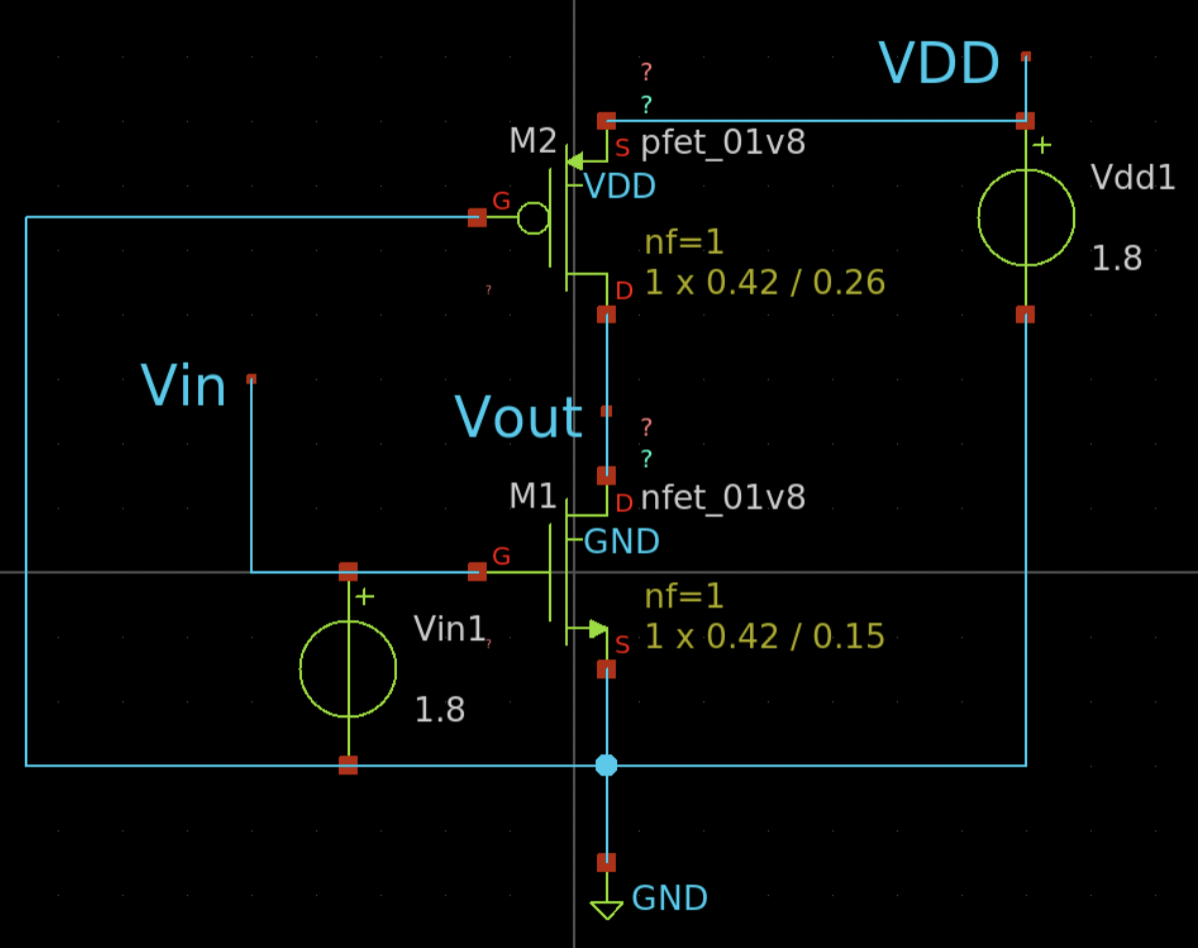
\includegraphics[scale=0.4]{tut2/reports/media/expt1.sch.png}
\end{center}


\subsection{Measurements}

We plot the voltage transfer charecteristics for the said inverter using a SPICE simulation and obtain the following plot:

\begin{center}
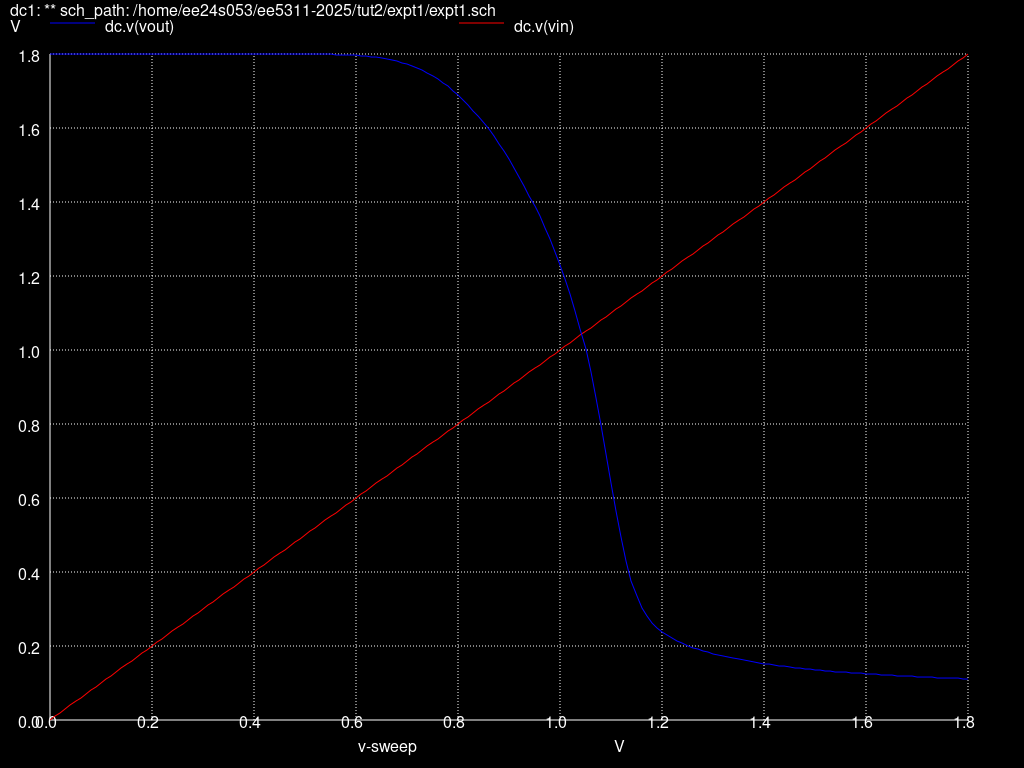
\includegraphics[scale=0.3]{tut2/reports/media/expt1_vtc.png}
\end{center}

We measure the inverter threshold voltage, defined as the magnitude of input voltage for which the output voltage is half of the supply voltage, as follows:

\begin{verbatim}
    meas dc Vtinv when v(Vout)=0.9 cross=1
\end{verbatim}

We observe that the inverter voltage is: $1.06587$ V.\newline
We also plot the first-order derivative of the output voltage curve using a SPICE simulation and obtain the following plot:

\begin{center}
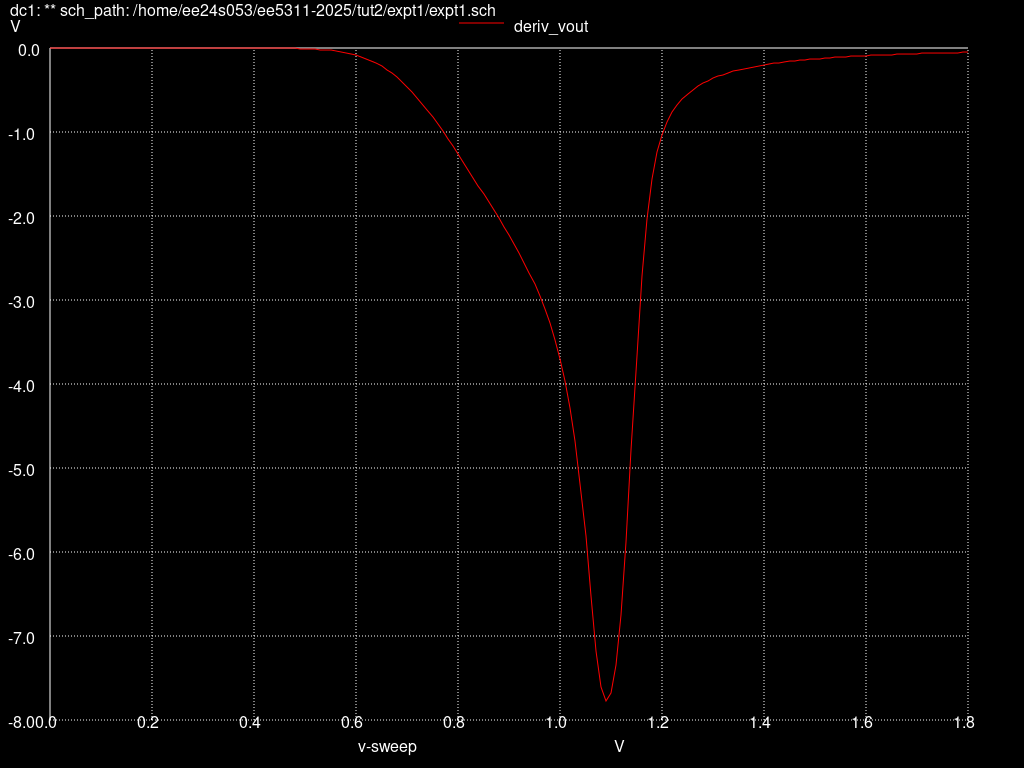
\includegraphics[scale=0.3]{tut2/reports/media/expt1_deriv_vout.png}
\end{center}

We measure the input voltage levels, $Vil, Vih$, as follows:

\begin{verbatim}
    let deriv_vout = deriv(v(Vout))
    meas dc Vil when deriv_vout=-1 cross=1
    meas dc Vih when deriv_vout=-1 cross=2
\end{verbatim}

We obtain the following values:

\begin{verbatim}
vil                 =  7.707750e-01
vih                 =  1.202181e+00
\end{verbatim}

Using these values for $Vil, Vih$, we compute the noise margins, $NM_{L}$ and $NM_{H}$ to be:

\begin{verbatim}
NML: 0.770775
NMH: 0.597819
\end{verbatim}

avg power is incomplete - need to figure out how to do that.

\section*{Experiment 02}
\subsection*{Calculations}
\subsection*{Schematics}
\subsection*{Measurements}

\section*{Declaration of AI Usage}

\end{document}
